\chapter{ルーズカップリングに基づくLIO}
\label{sec:loose_coupling_lio}

\section{状態量と問題設定}
\label{eq:state_and_problem_setting_loose_coupling}

前章で述べたスキャンマッチングでは,姿勢$T \in {\rm SE}(3)$のみを求める問題を考えていました.
これに対して本章で述べるLIOでは,以下の状態量を求めることを考えます.
%
\begin{align}
  {\bf x} = \left( {}^{O}{\bf t}_{I} ~ {}^{O}R_{I} ~ {}^{O}{\bf v} ~ {\bf b}^{\omega} ~ {\bf b}^{a} \right)
  \label{eq:loose_coupling_lio_state}
\end{align}
%
ここで${}^{O}{\bf t}_{I} \in \mathbb{R}^{3}$と${}^{O}R_{I} \in {\rm SO}(3)$は,オドメトリ座標でのIMUの姿勢を表す並進ベクトルと回転行列,${}^{O}{\bf v} \in \mathbb{R}^{3}$はオドメトリ座標系におけるIMUの速度ベクトル,${\bf b}^{\omega}, {\bf b}^{a} \in \mathbb{R}^{3}$はIMUの角速度と加速度に対するバイアスになります.
なお,$\left( \log \left( R \right) \right)^{\vee} \in \mathbb{R}^{3}$となるので,本章で述べるLIOでは15次元の状態を推定する問題となります.
また,IMUの姿勢を求めていることに注意してください.

LIOではLiDARとIMUを用いるため,各センサデータの時間軸を考えることが重要になります.
例えばLiDARが時刻$t-1$および$t$において,それぞれ$\mathcal{P}_{t-1}$,$\mathcal{P}_{t}$の点群を取得するとします.
この間,IMUは$\mathcal{U}_{t} = \left( \boldsymbol \omega_{t}^{1} ~ {\bf a}_{t}^{1} ~ \cdots ~ \boldsymbol \omega_{t}^{M_{t}} ~ {\bf a}_{t}^{M_{t}} \right)$のデータを計測するとします\footnote{一般にIMUの方がLiDARより計測周期が高いため,LiDARが計測を行う間にIMUの計測値は複数個存在します.}.
なお図\ref{fig:time_relationships}に,これらのセンサデータ,および本章で使われる時間の関係を図示しています.

本章で解説するLIOでは,LiDARとIMUの計測値を用いて,式(\ref{eq:loose_coupling_lio_state})に示す状態量を求めることが目標になり,これは以下の処理を繰り返すことで達成されます.
%
\begin{enumerate}
  \item IMUプレインテグレーションを用いた状態の予測
  \item LiDAR点群の歪み補正
  \item 局所地図とLiDAR点群のスキャンマッチング
  \item 予測およびスキャンマッチングの結果に基づく状態の再更新
  \item キーフレームの検出と局所地図の構築
\end{enumerate}
%
なお4の再更新の部分がルーズカップリングに相当し,これにはDirectLIO~\cite{DirectLIO}で用いられているHierarchical Geometric Observer(HGO)\cite{Lopez2023arXiv}を用います.
ただしHGOの利用がルーズカップリングとして良い方法であるということではなく,実装が用意なので紹介しているということに留意ください.
実装できるなら,拡張カルマンフィルたのような実装をするほうが良いといえます.

\begin{figure}[!t]
  \centering
  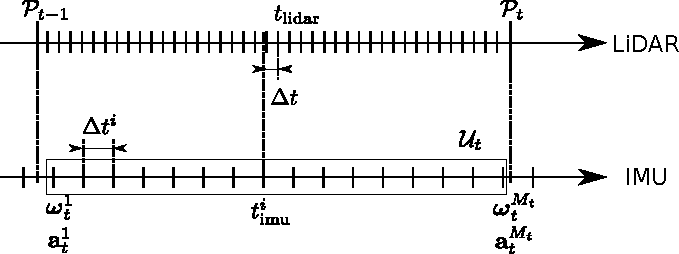
\includegraphics[width=0.6\textwidth]{../figs/time_relationships.pdf}
  \caption{Temporal relationship between LiDAR and IMU measurements.}
  \label{fig:time_relationships}
\end{figure}
















\section{IMUプレインテグレーション}
\label{subsec:imu_preintegration}

今時刻$t-1$の状態${\bf x}_{t-1}$まで推定が行われていて,時刻$t$のIMUのデータ$\mathcal{U}_{t}$が得られているとします.
スキャンマッチングを実行するにあたり,{\bf IMUプレインテグレーション}(IMU Preitegration)を用いて,回転行列,並進ベクトル,および速度ベクトルを以下のように更新します.
%
\begin{align}
  \begin{gathered}
    {}^{O}{\bf t}_{I, t} = {}^{O}{\bf t}_{I, t-1} + \sum_{i=1}^{M_{t}} {}^{O}{\bf v}_{t-1}^{j} \Delta t^{i} + \frac{1}{2} {}^{O}R_{I, t-1}^{j} \left( {\bf a}_{t}^{i} - {\bf b}_{t-1}^{a} \right) \left( \Delta t^{i} \right)^{2} + \frac{1}{2} {\bf g} \left( \Delta t^{i} \right)^{2} \\
%
    {}^{O}R_{I, t} = {}^{O}R_{I, t-1} \prod_{i=1}^{M_{t}} \exp \left( \left( \boldsymbol \omega_{t}^{i} - {\bf b}_{t-1}^{\omega} \right)^{\wedge} \Delta t^{i} \right) \\
%
    {}^{O}{\bf v}_{t} = {}^{O}{\bf v}_{t-1} + \sum_{i=1}^{M_{t}} {}^{O}R_{I, t-1}^{j} \left( {\bf a}_{t}^{i} - {\bf b}_{t-1}^{a} \right) \Delta t^{i} + {\bf g} \Delta t^{i} \\
  \end{gathered}
  \label{eq:discrete_imu_preintegration}
\end{align}
%
ここで${\bf g}$は重力加速度ベクトル,$\Delta t^{i}$は$i$番目から$i-1$番目のIMUの計測時間の差,${}^{O}R_{I, t-1}^{j}$と${}^{O}{\bf v}_{I, t-1}^{j}$はそれぞれ以下となります.
\begin{align}
  \begin{gathered}
    {}^{O}R_{I, t-1}^{j} = {}^{O}R_{I, t-1} \prod_{i=1}^{j} \exp \left( \left( \boldsymbol \omega_{t}^{i} - {\bf b}_{t-1}^{\omega} \right)^{\wedge} \Delta t^{i} \right) \\
%
    {}^{O}{\bf v}_{t-1}^{j} = {}^{O}{\bf v}_{t-1} + \sum_{i=1}^{j} {}^{O}R_{I, t-1}^{j} \left( {\bf a}_{t}^{i} - {\bf b}_{t-1}^{a} \right) \Delta t^{i} + {\bf g} \Delta t^{i} \\
  \end{gathered}
\end{align}
%
次に示すスキャンマッチングでは,式(\ref{eq:discrete_imu_preintegration})に示す並進ベクトルと回転行列を初期値として用います.
















\section{歪み補正}
\label{subsec:deskew_scan_distortion}

一般的にIMUの計測周期はLiDARの計測周期より高いです.
そのため,LiDARが1周期分の点群を計測する間に,複数のIMUの計測値を取得することが可能です.
そしてこの計測値を利用すると,式(\ref{eq:discrete_imu_preintegration})に示すように,LiDARが1周期分の点群を取得する間の姿勢を計算することができます.
そしてこれらの姿勢を利用すると,LiDARが計測した各点をより正確な位置に補正することができます.
この操作を,LiDARのデータの歪み補正と呼びます.

歪み補正の解説を行う前に,まずIMUプレインテグレーションにより得られた$M_{t}+1$個の姿勢の集合を$\left( {}^{O}T_{I}^{0}, \cdots, {}^{O}T_{I}^{M_{t}} \right)$とし,またこれらの姿勢列に対応した$M_{t}+1$個の時間の集合を$\left( t_{\rm imu}^{0}, \cdots, t_{\rm imu}^{M_{t}} \right)$とします.
なお,${}^{O}T_{I}^{j} = \left( {}^{O}R_{I, t-1}^{j} \mid {}^{O}{\bf t}_{I, t-1}^{j} \right) \in {\rm SE}(3)$です.
また,${}^{O}T_{I}^{0} = {}^{O}T_{I, t-1}$,${}^{O}T_{I}^{M_{t}} = {}^{O}T_{I, t}$となります.

歪み補正を行う前提として,LiDARが計測した各点にタイムスタンプが付与されていることを前提とします.
そしてこのタイムスタンプを用いて,$t_{\rm imu}^{i} \leq t_{\rm lidar} \leq t_{\rm imu}^{i+1} ~ \left( i = 0, \cdots, M_{t}-1 \right)$となるIMUの計測値を探索します.
今,$i$番目と$i+1$番目の時間の間でLiDARが点${}^{L}{\bf p}$を計測していたとします.
このとき,この点を計測した際のIMUの姿勢を以下のように求めます.
%
\begin{align}
  \begin{gathered}
    \Delta t = t_{\rm lidar} - t_{\rm imu}^{i} \\
%
    {}^{O}R_{I}^{d} = {}^{O}R_{I, t-1}^{i} \exp \left( \left( \boldsymbol \omega_{t}^{i} - {\bf b}_{t-1}^{\omega} 
\right)^{\wedge} \Delta t \right) \\
%
    {}^{O}{\bf t}_{I}^{d} = {}^{O}{\bf t}_{I, t-1}^{i} + {}^{O}{\bf v}_{t-1}^{i} \Delta t + \frac{1}{2} {}^{O}R_{I, t-1}^{i} \left( {\bf a}_{t}^{i} - {\bf b}_{t-1}^{a} \right) \Delta t^{2} + \frac{1}{2} {\bf g} \Delta t^{2}
  \end{gathered}
\end{align}
%
そして,${}^{O}T_{I}^{d} = \left( {}^{O}R_{I}^{d} \mid {}^{O}{\bf t}_{I}^{d} \right)$を定め,${}^{L}{\bf p}$を以下のようにIMU座標の点に変換します.
%
\begin{align}
  {}^{I}{\bf p} = \left( {}^{O}T_{I}^{M_{t}} \right)^{-1} {}^{O}T_{I}^{d} {}^{I}T_{L} {}^{L}{\bf p}
\end{align}
%
ここで${}^{I}T_{L}$はLiDARとIMU間の剛体変換を表す行列であり,事前に求められているものとしています.
この操作をすべての計測点群に対して行うことで,LiDARが計測した点群の歪みを補正することができます.
なお一番最後に$\left( {}^{O}T_{I}^{M_{t}} \right)^{-1}$を適用することで,式(\ref{eq:discrete_imu_preintegration})で予測したIMUの姿勢を原点とした座標の点群が得られます.


















\section{局所地図とのスキャンマッチング}

IMUプレインテグレーションによる予測,および歪み補正を終えた後に,{\bf 局所地図}(Local Map)とのスキャンマッチングを実施します.
なお説明の都合上先に局所地図とのスキャンマッチングについて述べますが,局所地図の作成方法に関しては\ref{subsec:local_map_building}節で述べます.
またスキャンマッチングに関しては基本的に\ref{sec:scan_matching}章で述べた方法を用いますが,本節では使用されるデータや座標に関して整理しておきます.

まず局所地図を表す点群${}^{O}\mathcal{M}$が,オドメトリ座標上で構築されているとします\footnote{局所座標の構築方法にも様々な方法があり,明示的にオドメトリ座標で地図構築を行わない方法もあります.}.
また前節で述べた歪み補正も適用され,LiDARの計測点群はIMU座標での点群${}^{I}\mathcal{P}$が得られているとします.
このとき,LiDARの計測点${}^{I}{\bf p}$に対する残差ベクトルを以下のように定めます.
%
\begin{align}
  {\bf r} = {}^{O}{\bf q} - {}^{O}T_{I} {}^{I}{\bf p}
  \label{eq:residual_vector_lio_scan_matching}
\end{align}
%
なお${}^{O}{\bf q}$は,${}^{O}\mathcal{M}$の点で${}^{O}T_{I} {}^{I}{\bf p}$に最も近い点です.
そして,以下に示すコスト関数の最小化を行います.
%
\begin{align}
  E \left( {}^{O}T_{I} \right) = \sum_{i=1}^{N} \rho \left( \left\| {\bf n}_{i}^{\top} {\bf r}_{i} \right\|_{2}^{2} \right)
  \label{eq:cost_function_lio_scan_matching}
\end{align}
%
ただし${\bf n}$は,${}^{O}{\bf q}$に対応する法線ベクトルになります.















\section{ルーズカップリングによる状態量の更新}

IMUプレインテグレーションにより予測された姿勢を${}^{O}\hat{T}_{I}$,スキャンマッチングにより得られた姿勢を${}^{O}T_{I}^{*}$とします.
またこれらに対応する並進ベクトルと回転行列に対応するクォータニオンをそれぞれ${}^{O}\hat{ {\bf t} }_{I}$,${}^{O}{\bf t}_{I}^{*}$,${}^{O}\hat{ {\bf q} }_{I}$,${}^{O}{\bf q}_{I}^{*}$とします.
これらを用いて,最新の状態をそれぞれ以下のように更新します.
%
\begin{align}
  \begin{gathered}
    {}^{O}{\bf q}_{I} = {}^{O}\hat{ {\bf q} }_{I} + \Delta t \gamma_{1} {}^{O}\hat{ {\bf q} }_{I} \left( \begin{matrix} 1 - \left| q_{w}^{d} \right| \\ {\rm sgn} \left( q_{w}^{d} \right) {\bf q}_{v}^{d} \end{matrix} \right) \\
    {\bf b}^{\omega} = \hat{ {\bf b} }^{\omega} - \Delta t \gamma_{2} q_{w}^{d} {\bf q}_{v}^{d} \\
    {}^{O}{\bf t}_{I} = {}^{O}\hat{ {\bf t} }_{I} + \Delta t \gamma_{3} {\bf t}^{d} \\
    {}^{O}{\bf v} = {}^{O}\hat{ {\bf v} }_{t} + \Delta t \gamma_{4} {\bf t}^{d} \\
    {\bf b}^{a} = \hat{ {\bf b} }^{a} - \Delta t \gamma_{5} {}^{O}\hat{R}_{I}^{\top} {\bf t}^{d}
  \end{gathered}
\end{align}
%
ここで$\Delta t$はIMUプレインテグレーションを行った時間の総和,$\gamma_{1-5}$は任意の正の定数,${\bf q}^{d} = {}^{O}\hat{ {\bf q} }_{I}^{-1} \otimes {}^{O}{\bf q}_{I}^{*}$,${\bf t}^{d} = {}^{O}{\bf t}_{I}^{*} - {}^{O}\hat{ {\bf t} }_{I}$です.
また${\bf q}^{d} = \left( q_{w}^{d} ~ \left( {\bf q}_{v}^{d} \right)^{\top} \right)^{\top}$,${\bf q}_{v}^{d} = \left( q_{x}^{d} ~ q_{y}^{d} ~ q_{z}^{d} \right)^{\top}$であり,${}^{O}\hat{R}_{I}$は${}^{O}\hat{ {\bf q} }_{I}$に対応する回転行列です.



















\section{局所地図の構築}
\label{subsec:local_map_building}

局所地図を構築する方法も様々ありますが,本書ではキーフレームを用いた方法を採用します.
具体的には,LIOが推定する姿勢の中からいくつかの姿勢をキーフレームとして選択し,その姿勢とそれに対応するLiDARの点群を用いて局所地図${}^{O}\mathcal{M}$の作成を行います.
キーフレームの検出にあたっては,最も単純な方法ではありますが,移動量に対して閾値を設け,前回検出したキーフレームからの並進移動量,もしくは回転量が一定値を超えた場合に,新たにキーフレームとして検出を行います.

今キーフレームの集合として$\left( {}^{O}T_{I, 1}, \cdots, {}^{O}T_{I, K} \right)$,またこれらのキーフレームに対応したLiDARの点群$\left( {}^{I}\mathcal{P}_{1}, \cdots, {}^{I}\mathcal{P}_{K} \right)$があるとします.
なお$K$は局所地図を構築するために使用するキーフレームの数です.
これらの点すべてを対応するキーフレームでオドメトリ座標に変換した点の集合を局所地図として定めます.
%
\begin{align}
  {}^{O}\mathcal{M} = \bigcup_{i=1}^{K} \bigcup_{{}^{I}{\bf p} \in {}^{I}\mathcal{P}_{i}} {}^{O}T_{I, i} {}^{I}{\bf p}
\end{align}
%

キーフレームをいくつ利用するかにもよりますが,通常局所地図は大きな点群となります.
そのため,すべての点に対して法線ベクトルを計算すると非常に大きな計算コストが発生します.
また局所地図が大きくなると,スキャンマッチングに使用されない点も多く含まれてきます.
そのため本実装では,式(\ref{eq:residual_vector_lio_scan_matching})に示す残差ベクトルが定義されたときに,その点に対応する法線ベクトルの計算を行うことにします.
また,計算済みかどうかを判定するフラグも実装し,局所地図構築に関する計算コストの削減を行っています.















\section{実用にあたって}

ルーズカップリングに基づくLIOは,次章で述べるタイトカップリングに基づくLIOと比較すると,実装やパラメータ調整が容易に行うことができます.
加えて,おおよその環境では十分な性能を持って機能します.
そのため,まずLIOを実装し,LiDARとIMUを融合させる方法を知りたいという方には,適した手法であるといえます.
ただし多くの場合,タイトカップリングに基づくLIOの方が精度が高い傾向にあります.
ただしタイトカップリングに基づくLIOは実装やパラメータ調整の難易度が上がります.
繰り返しにはなりますが,ルーズカップリングに基づくLIOも十分な性能を持つため,ルーズカップリングが良いかタイトカップリングが良いかは,ユーザーの状況次第になるといえます.

LIOで最も計算コストがかかる部分は,局所地図の構築部分になります.
局所地図はサイズを小さくすれば構築の計算コストは下がりますが,その分スキャンマッチングに利用できる範囲が限定されるため,移動量推定においてドリフト誤差が発生しやすくなってしまいます.
しかし局所地図のサイズを大きくしすぎると,地図構築の計算コストが増大し,最悪の場合,LiDARの計測周期を超えるような計算時間となり,LIOの破綻に繋がってしまいます.

また局所地図の更新頻度もLIOの精度に大きく関わります.
特にLiDARの観測がスキャンマッチングに適さないような環境では,できる限り局所地図を更新する頻度を向上させた方がLIOの精度を維持することができます.
しかし当然ながら,局所地図の更新頻度が増えるほど計算コストの増大にも繋がります.
また本実装では,単純な移動量に対して閾値を設けて局所地図の更新をおこなっているため,局所地図の更新頻度を高くすると,局所地図として地図化できる範囲が小さくなり,これもドリフト誤差を発生させやすくなる要因になります.
LIOの精度が低下する場合などは,局所地図に関するパラメータの調整,またもしくは,局所地図の更新ルールを見直すことが効果的なことが多いです.
なおこれらの局所地図に関する問題は,次章で述べるタイトカップリングに基づくLIOでも同様に表れます.



















